

\begin{problem}{Минимизируй SokoBan}{Входные данные}{Результат}{}

Sokoban (Soko-Ban, яп.~--- «кладовщик»)~--- логическая игра-головоломка, в которой игрок передвигает ящики по лабиринту, показанному в виде плана, с целью поставить все ящики на заданные конечные позиции. 


Для этого пользователь перемещает человека, которого мы называем Сокобан. Сокобан может двигаться вверх, вниз, влево и вправо. Он не может проходить сквозь стены или ящики. Он может толкать только одну коробку за раз (никогда не тянуть). В любое время квадрат может быть занят только одной стеной, коробкой или Сокобаном.

Более формально, вам изначально известная конфигурация лабиринта~--- поля $n\times m$, состоящая из пустых клеток или стен. Также вам известна начальная позиция каждого из ящиков, конечные позиции, куда надо поставить ящики и начальное положение Сокобана.



\InputFile
Входной файл содержит на первой строке одно число $t$~--- число различных тестовых данных. Затем следует $t$ описаний тестов. Описание $i$-го теста в первой своей строке содержит два числа $n_i$ и $m_i$, описывающие размер поля. Далее следует описание лабиринта: $n_i$ строк по $m_i$ символов в каждой. \texttt{<<.>>} означает, что клетка свободна; $\texttt{<<\#>>}$, что в клетке находится стена. на следующей строке вводятся два числа $x_s$, $y_s$~--- начальные координаты Сокобана, означающие, что он находится в $x_s$-м ряду, в $y_s$-м столбце. На следующей строке находится число $k$~--- количество коробок на игровом поле. Следущие $k$ строк содержат по два числа $x_{bi}$, $y_{bi}$ ~--- начальные координаты $i$-й коробки.
Следущие $k$ строк содержат по два числа $x_{ti}$, $y_{ti}$ ~--- координаты $i$-й позиции, в которой можно оставить коробку.
Нумерация координат начинается с единицы. Гарантируется, что начальная конфигурация соответствует правилам, то есть, все коробки, стены и Сокобан находятся на разнх клетках

\OutputFile
Для каждого из $t$ тестов выведите ответ в следующем формате: в первой строке выведите $ans_i$~--- число ходов, необходимое чтобы решить уровень, либо 0, если вы не смогли найти решение. Затем выведите $ans_i$ строк, показывающих последовательность ходов, необходимую для победы: выведите \texttt{<<Up>>}, чтобы обозначть перемещение Сокобана вверх, \texttt{<<Down>>}~--- вниз, \texttt{<<Left>>}~--- влево, \texttt{<<Right>>}~--- вправо.


{\noindent\bf\problemsectionfont\textsf{Система оценки}}

Оценка за каждый тест вычисляется по формуле $2 \times\left(\frac{\text {BestSolution}}{\text {ParticipantSolution}}\right)^{4}$, где $\text{ParticipantSolution}$~--- длина пути, найденного участником, а $\text{BestSolution}$~--- длина пути в лучшем среди участников и жюри решении.

Оценка за группу тестов является суммой оценок по тестам данной группы.

В первой группе тестов $t = 15$. Максимальная оценка за эту группу: $30$ баллов. 

Во второй группе тестов $t = 35$. Максимальная оценка за эту группу: $70$ баллов. Во время тура проверяется. что сданный файл соответствует формату выходных данных чисел. Проверка правильности ответа осуществляется в режиме offline (результат виден после окончания тура).

Если ответ на хотя бы один из тестов группы не удовлетворяет описанному выше формату, решение получит 0 баллов. 

{\noindent\bf\problemsectionfont\textsf{Примечания}}

Ниже приведён пример решения теста из условия за 21 ход.

\begin{figure}
   \makebox[\linewidth][c]{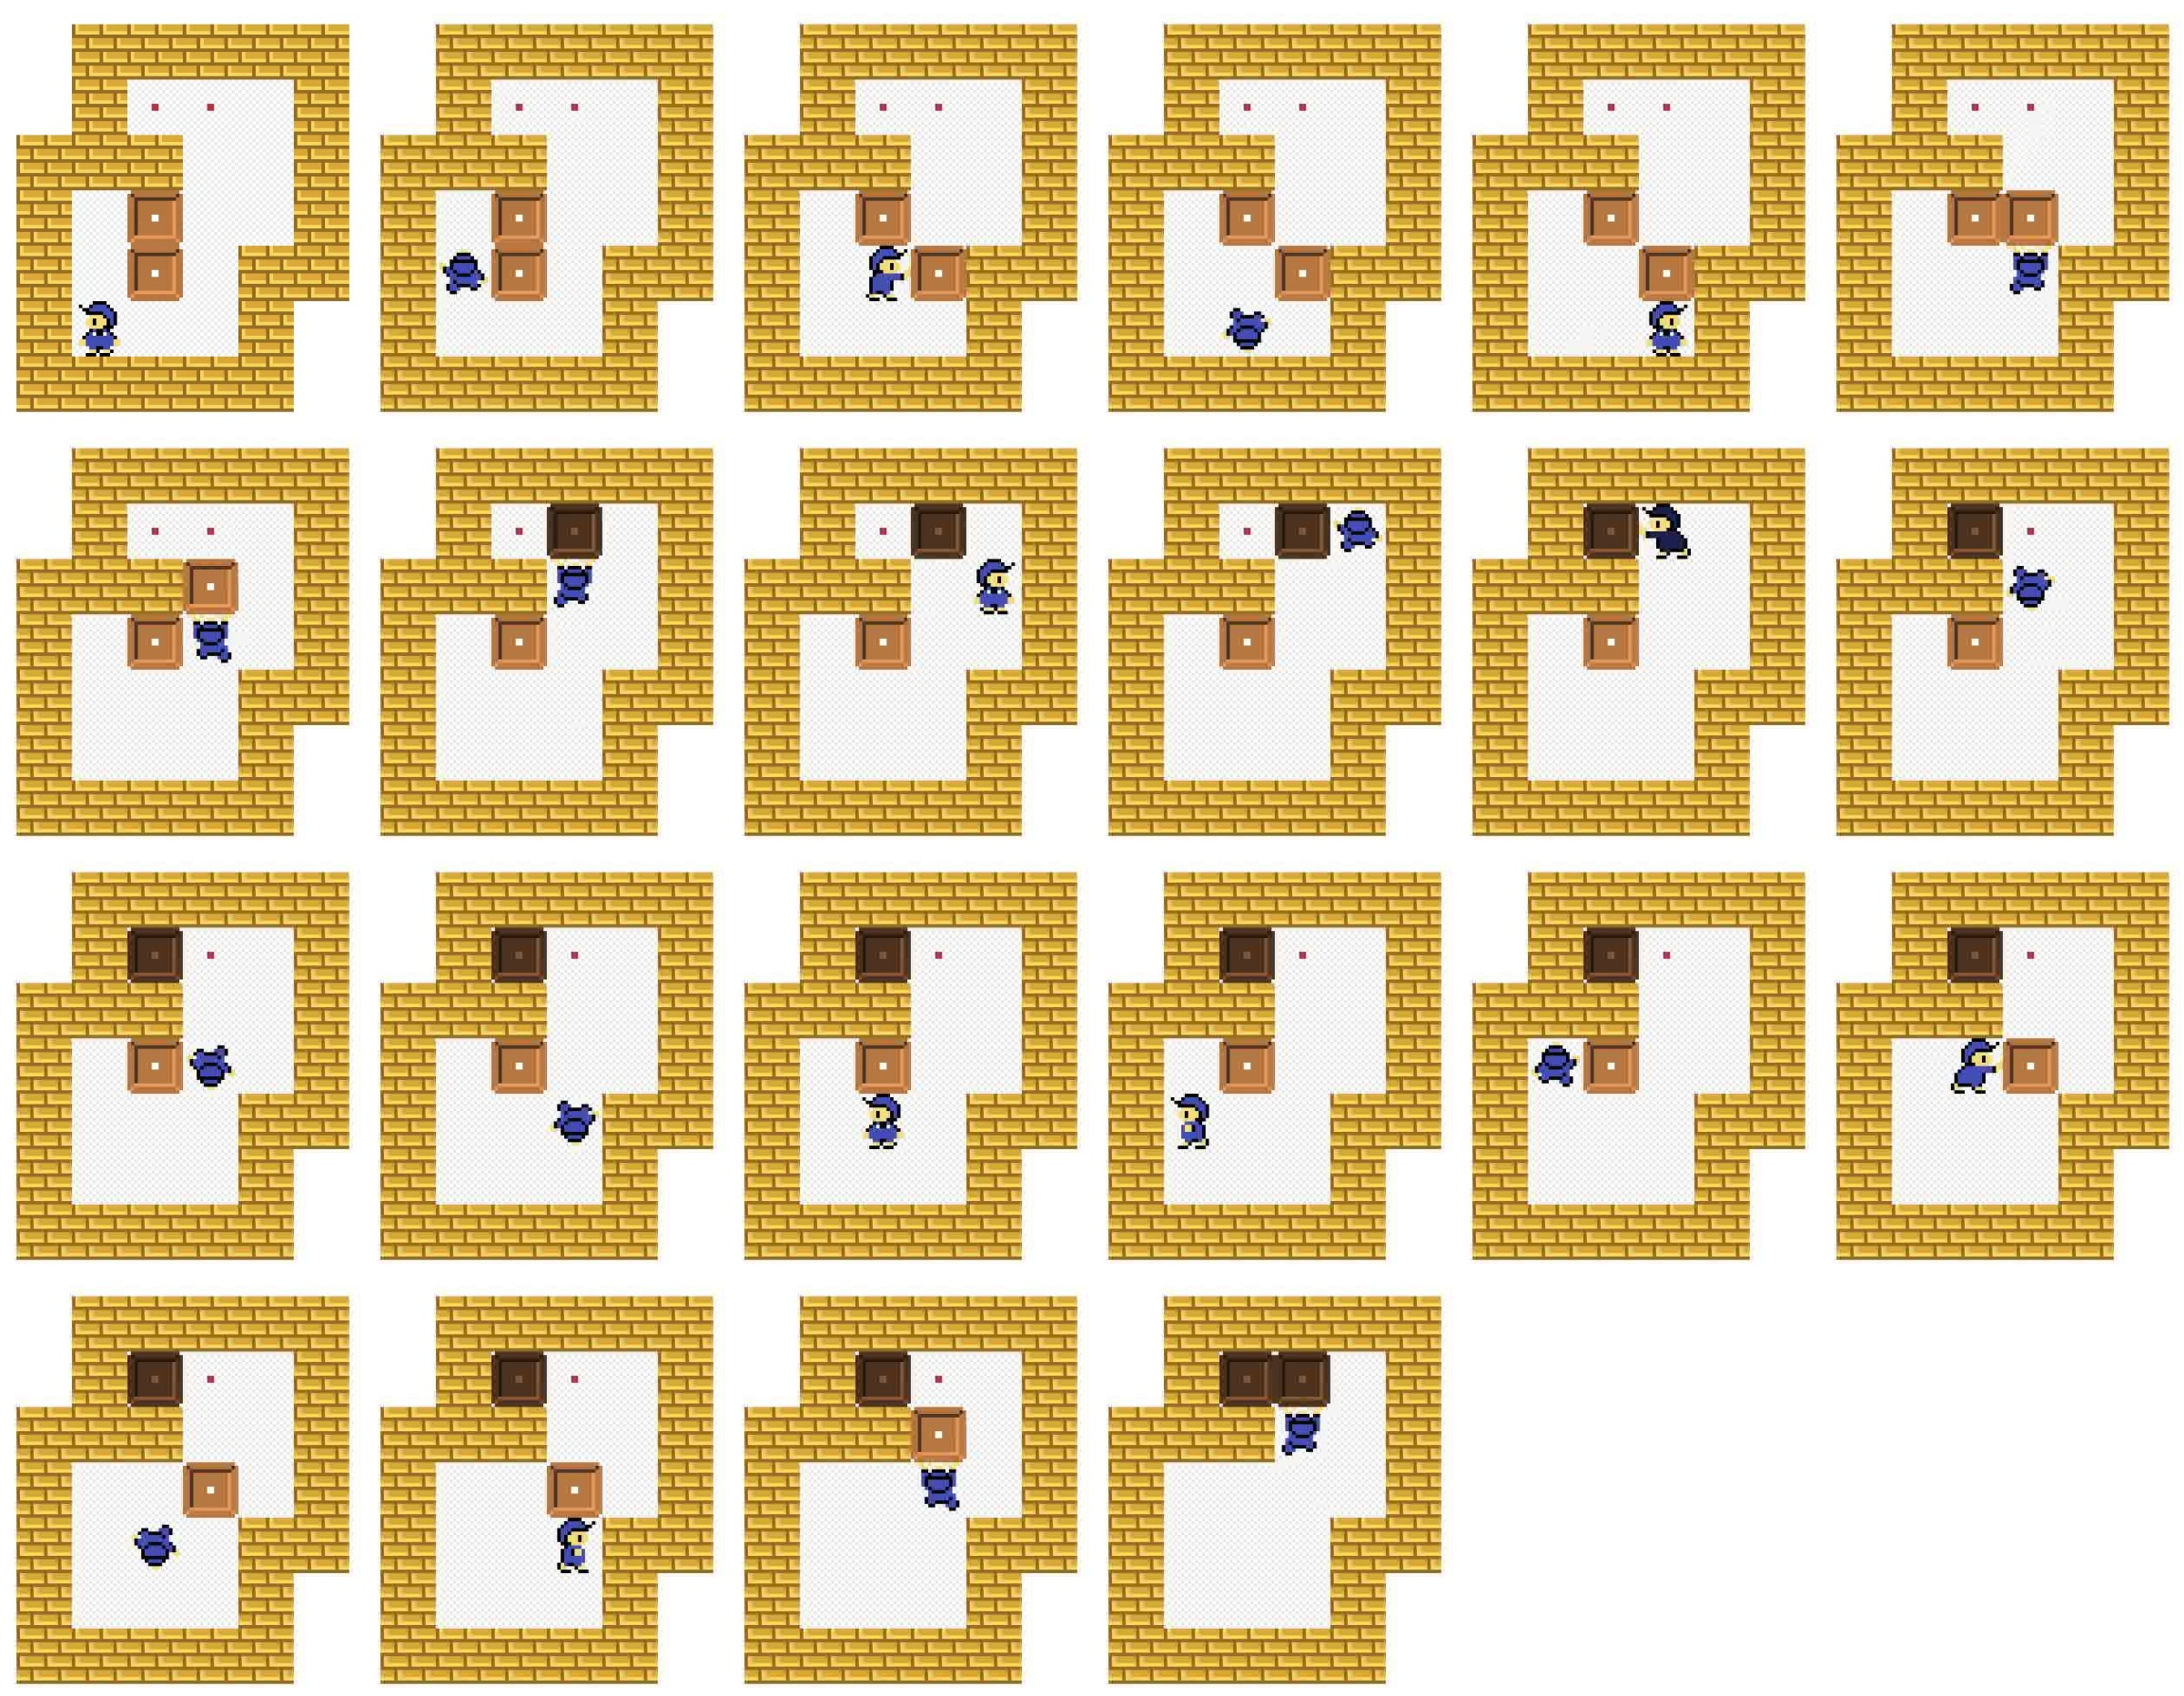
\includegraphics[width=0.8\textwidth]{example-sokoban.jpg}}
\end{figure}


\Examples
\begin{example}
\exmp{
1
7 6
\#\#\#\#\#\#
\#\#...\#
\#\#\#..\#
\#....\#
\#...\#\#
\#...\#\#
\#\#\#\#\#\#
6 2
2
4 3
5 3
2 3
2 4
}{
21
Up
Right
Down
Right
Up
Up
Up
Right
Up
Left
Down
Down
Down
Left
Left
Up
Right
Down
Right
Up
Up
}%
\end{example}


\end{problem} 


